% !TEX TS-program = LuaLaTeX

\documentclass{coderdojo}

\worksheet{11}{Building a GUI}

\newcommand\contentsitem[2]{
	\item \hyperref[#1]{\color{section}\bfseries #2}
}

\usepackage{wrapfig}
\usepackage{float}

\newcommand\TODO[1]{
\begin{itemize}
\item[\todoSymbol] \color{todo} #1
\end{itemize}}


\newcommand\TEST[1][\bf Test your code!]{
	\centerline{\tikz\node[starburst, fill=yellow, draw=red, line width=2pt,align=center] {#1};}
}

\newcommand\TESTSMALL[2][\bf Test your code!]{
{\tikz[scale=#2]\node[starburst, fill=yellow, draw=red, line width=2pt,align=center] {#1};}
}

\usetikzlibrary{decorations.pathreplacing}

\begin{document}
\maketitle


\section*{Introduction}

The title of this worksheet is a little ambitious --- we are not going build a full Graphical User Interface (GUI) but just a main menu with some (hopefully cool) features.  However, what we are going to do, is to develop everything ourselves (using turtle graphics) rather than using one of the many GUI libraries available in python. 

\vspace{6pt}
You could ask ``{\em Why?}'' as in ``{\em Why would we build our own menu system? Surely it is easier to use an existing GUI library?}''

\begin{minipage}{.5\textwidth}
The answer is: Yes, it would be easier, but we want to build our own because;

\begin{itemize}
\item We can.
\item We will use this to learn how GUI respond to events (mouse click, keyboard press/release, etc.).
\item We will be able to add our own special effects (more later) to our GUI.
\end{itemize}
\end{minipage}
\begin{minipage}{.5\textwidth}
\begin{figure}[H]
\centering
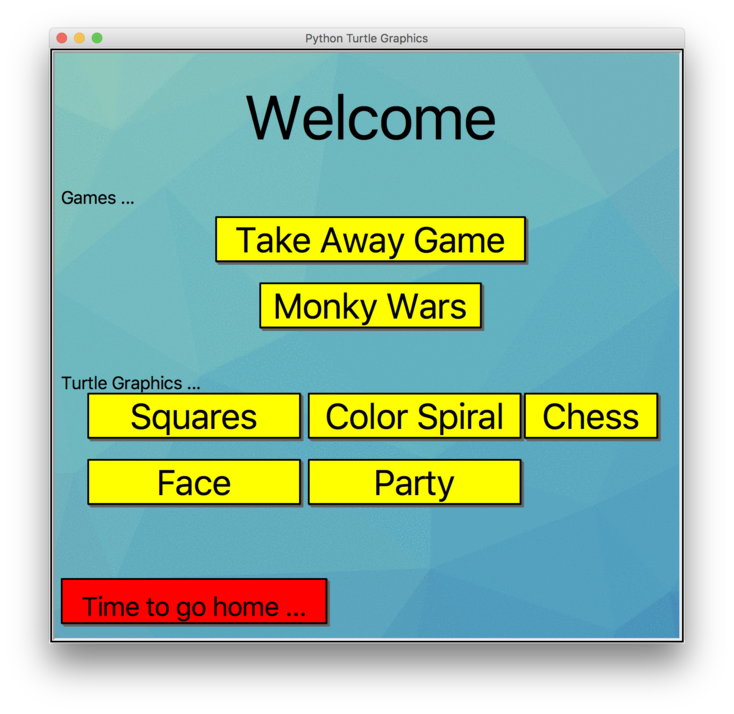
\includegraphics[width=6cm]{Menu_Complete}\\[-12pt]
\caption{Completed main menu.} 
\end{figure}
\end{minipage}

\vspace{6pt}
As usual we build this using a sequence of steps --- testing our code along the way.

\begin{dingautolist}{192} 
\contentsitem{screen}{Creating the Menu Screen}

We have done this many time before. All we need do is import the \code{turtle} module and create a \code{Screen} where we place our drawing, and a \code{Turtle} or two to do the actual drawing.  We do one thing that is new --- we insert a background image (must be in \code{gif} format).

\contentsitem{button}{Creating Buttons that Work}

Here we need to do some fancy coding --- both in drawing our buttons and figuring out how to respond to a button click.  

\contentsitem{take_away}{Building the Menu}

Finally, here you can design your menu screen anyway you want --- don't be stuck with my boring, everything is in a gird layout.

\contentsitem{button}{Updating our Earlier Programs so they Behave with Our Menu --- TODO}

We will need to modify some of our earlier programs (Graphical Take Away, Monkey Wars, etc) so they work better when we run them from our menu.  

This is a small task that we will leave until next week. Also we have yet to add the cool features!

\end{dingautolist}

\clearpage
\section{Creating the Menu Screen}\label{sec:screen}

\TODO{Create file called \code{Menu.py} and insert the following code.}

\codeonly{title={\code{Menu.py}}}{1}{120}{code}{Menu_Start.py}  
\mbox{}\hfill\raisebox{4cm}[0pt][0pt]{%
	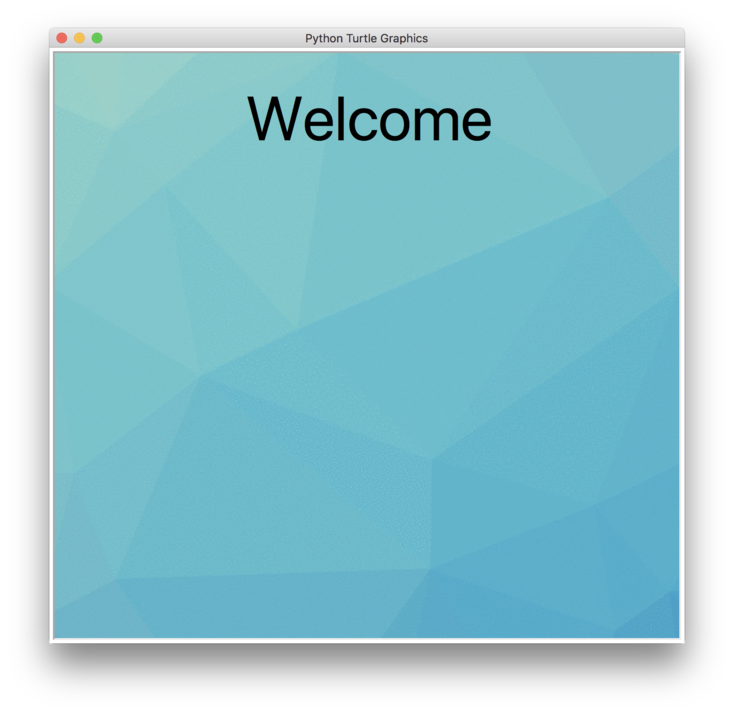
\includegraphics[width=9cm]{Menu_Start}
}\hspace*{-1.5cm}

Our code will get long so we need to keep things organised. Here the code is divided in to four sections --- import modules, create the empty screen and set background, define helper functions, and finally build the screen.

Currently this code just creates the window with the ``Welcome'' message. Next we will add buttons and mouse click events.
\clearpage

\section{Creating Buttons that Work}\label{sec:buttons}

\begin{figure}[H]
\centering\larger[2]\vspace{-18pt}
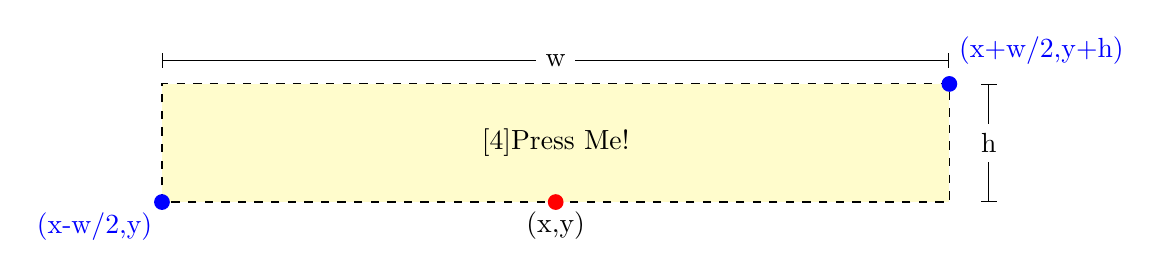
\begin{tikzpicture}
	\draw[dashed,fill=yellow!20] (-5,0) rectangle (5,1.5);
	\fill[red] (0,0) circle (.1) node[below,black] {(\code{x},\code{y})};
	
	\node[font={\larger[4]}]  at (0,0.75) {Press Me!};
	\draw[|-|] (5.5,0) -- node[fill=white] {\code{h}} ++(0,1.5); 
	\draw[|-|] (-5,1.8) -- node[fill=white] {\code{w}} ++(10,0); 
	\fill[blue] (-5,0) circle (.1) node[below,left,yshift=-9pt] {(\code{x}-\code{w/2},\code{y})};
	\fill[blue] (5,1.5) circle (.1) node[above,right,yshift=12pt] {(\code{x+w/2},\code{y+h})};
\end{tikzpicture}
\caption{Button position and dimensions.\label{fig:button}}
\end{figure}

\subsection{Developing a function to build a Button}

In order to create a button that we can click we need to decide on its:
\begin{itemize}
\item Position\footnote{Remember how we navigate across the screen
\begin{itemize}
\item
The centre, also called the {\bf origin}, and is denoted by $(0,0)$.
\item
Every point on the screen is defined by two numbers, $(x,y)$, where $x$ = how far to the right of the origin and $y$ = how far above the origin.
\end{itemize}} on the screen, (\code{x,y})

{\em We want the button text to be centred and draw the rectangle around the text so we will position a button based on the centre of the bottom edge (see Figure~\ref{fig:button})}.

\item Width, (\code{w}), and height, (\code{h}).

{\em
We need to draw a box big enough so that it looks like the text is inside this. If we used a GUI library this would be done automatically but we will do this manually and just pick numbers for now.}

\item Button label, (\code{label})

{\em This will be the text that the user sees and also the name of the button when we are responding to events.}

\item Font, (\code{font})

{\em
We might want the more important buttons to use a larger font so we need to be able to set this.}

\end{itemize}

Since we are planning to create multiple buttons we should write a function that we can call for every button.

\TODO{At the bottom of the ``\code{Define helper functions}''  section of your code insert the following function. }  

\codeonly{title={\code{Menu.py}}}{31}{38}{code}{Menu_1.py}  

In the above code, we have given default values for every parameter --- this will simplify our code later.

\TODO{After the ``Welcome'' message code in the ``\code{Build sceen}''  section, try to create a few buttons using the following code:} 
 
\codeonly{title={\code{Menu.py}}}{48}{50}{code}{Menu_1.py}  

\TODO{Run your code} 

You should see nothing on the screen, but see three messages in Thonny saying  

\begin{verbatim}
Button `Press Me` Not done yet
Button `No Press Me` Not done yet
Button `Forget them, PRESS ME` Not done yet
\end{verbatim}

Now we are going to implement our button function \ldots

\subsubsection{Draw the button label}

\vspace{6pt}

\TODO{After the  ``\code{draw label}'' comment insert code that jumps \code{bob} to correct position and writes the button label. Run this and you should see the labels.}

\codeonly{title={\code{Menu.py}}}{36}{38}{code}{Menu_2.py}  
\mbox{}\hfill\raisebox{0cm}[0pt][0pt]{%
	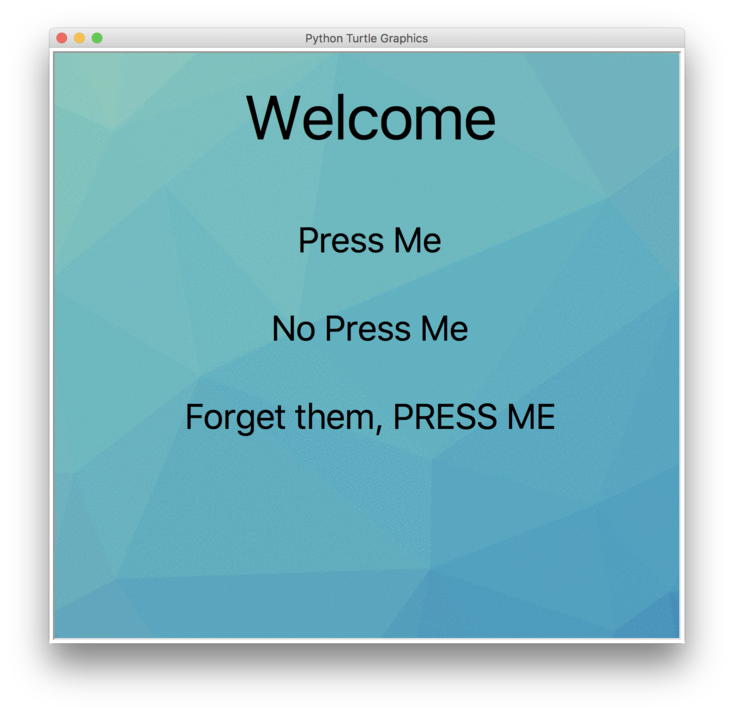
\includegraphics[width=4cm]{Menu_2}
}\hspace*{-1.5cm}

This looks good. Lets now add a border \ldots 

\subsubsection{Draw the border}

\TODO{After the  ``\code{draw border}'' comment insert code that draws a 
rectangle of width \code{w}, and height \code{h}}

\codeonly{title={\code{Menu.py}}}{40}{45}{code}{Menu_3.py}  
\mbox{}\hfill\raisebox{0.5cm}[0pt][0pt]{%
	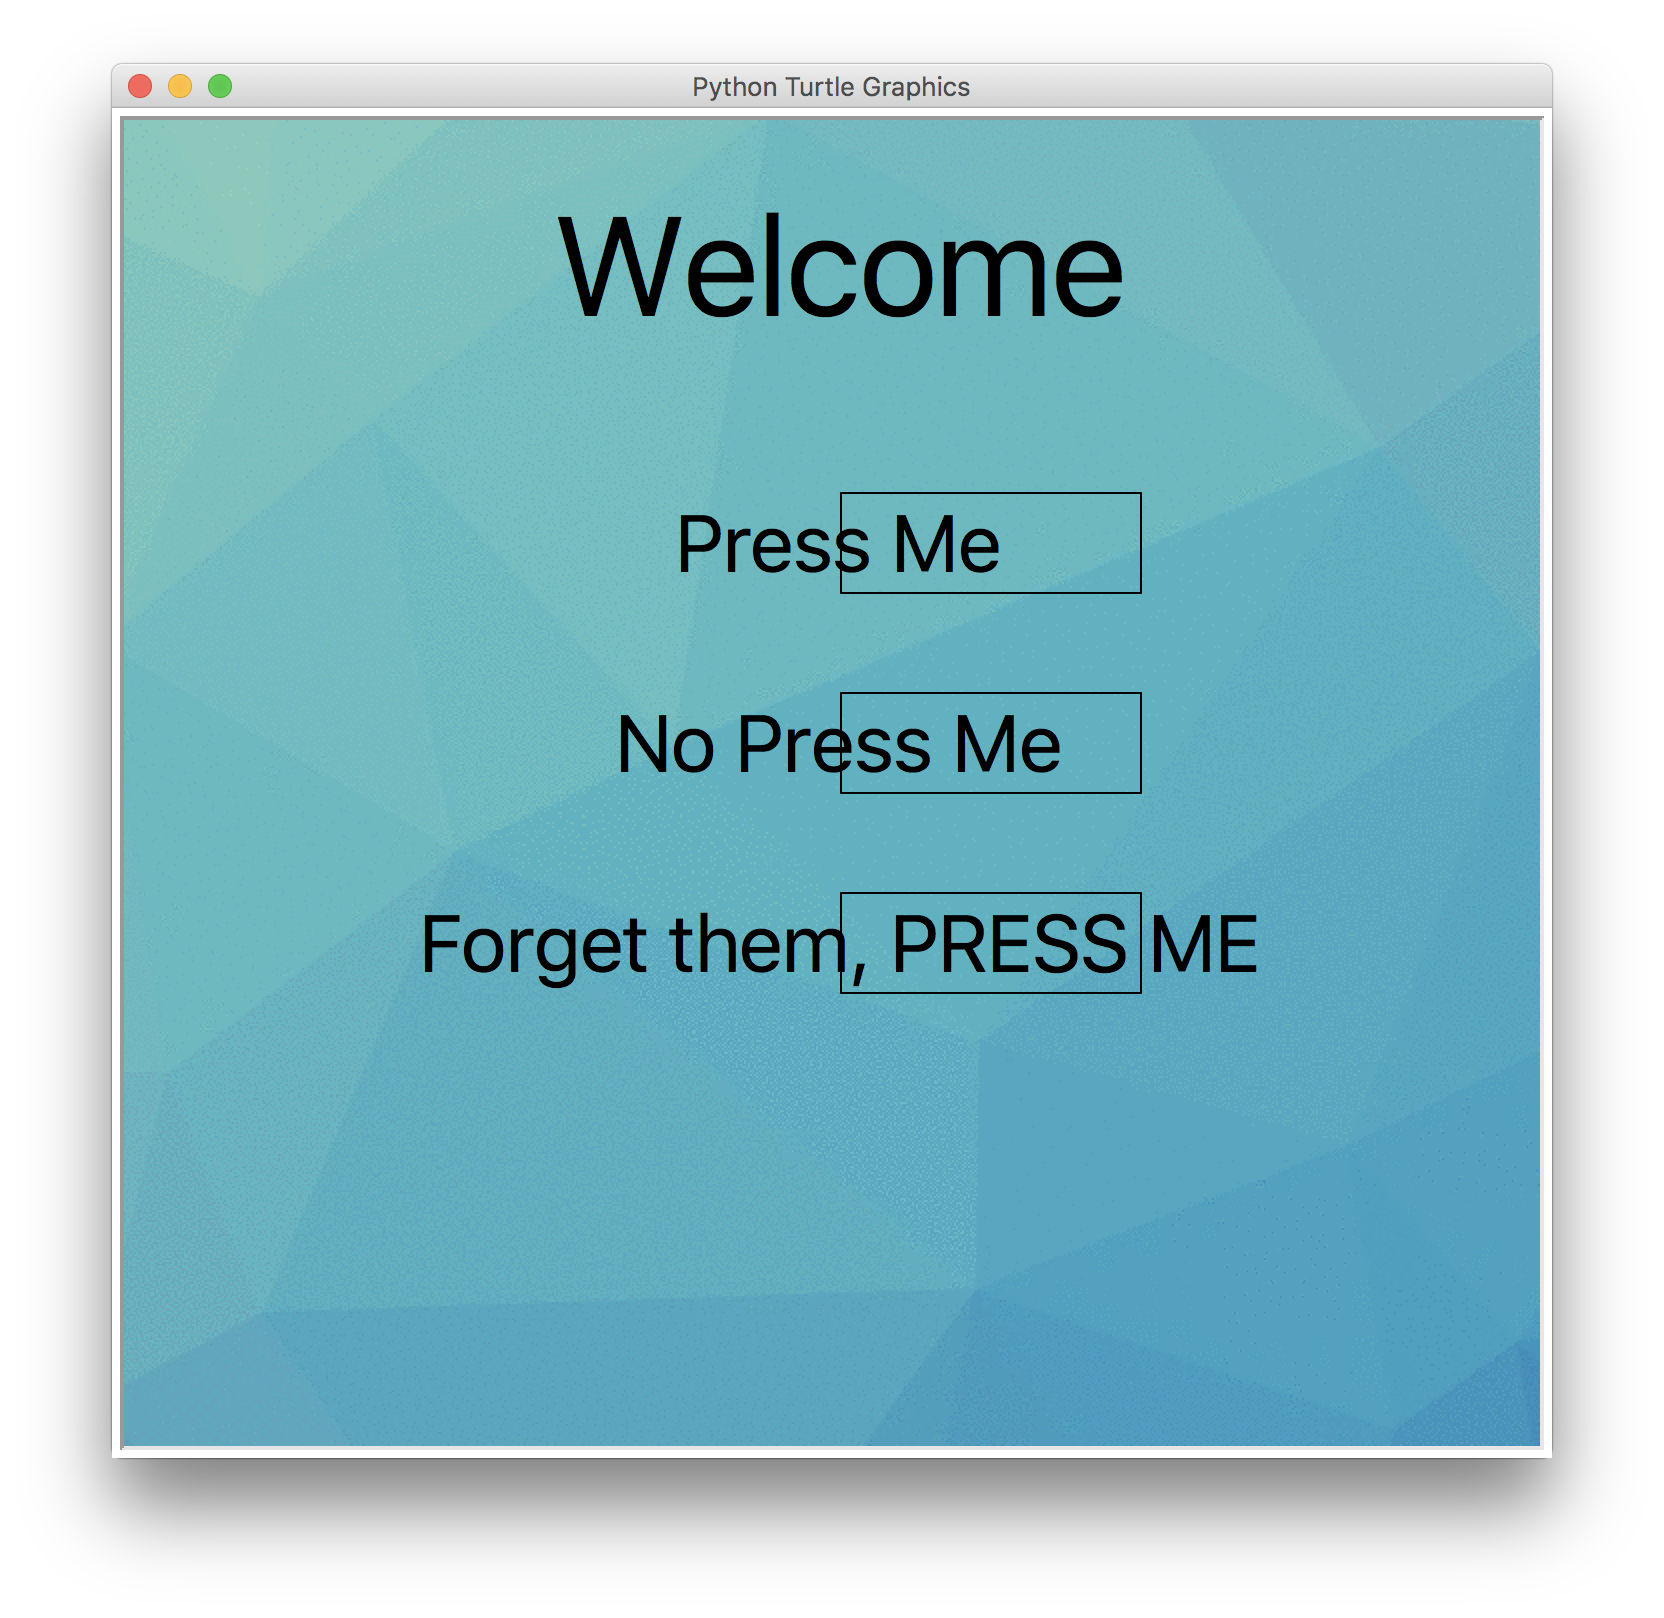
\includegraphics[width=4cm]{Menu_3}
}\hspace*{-1.5cm}

I see two problems here. The width of the rectangles is too small --- this is easy to fix. We just set the \code{w} parameter when calling \code{drawButton}. The second problem is that the rectangle is drawn starting from the bottom centre of the label --- we fix this by moving \code{bob} to the bottom left corner (see Figure~\ref{fig:button}).

\TODO{Insert code to move \code{bob} to bottom left corner, and change the widths of the 
button in your \code{drawButton} calls by setting parameter \code{w}. You should then get the following.}

\codeonly{title={\code{Menu.py}}}{40}{46}{code}{Menu_4.py}  
\mbox{}\hfill\raisebox{0.5cm}[0pt][0pt]{%
	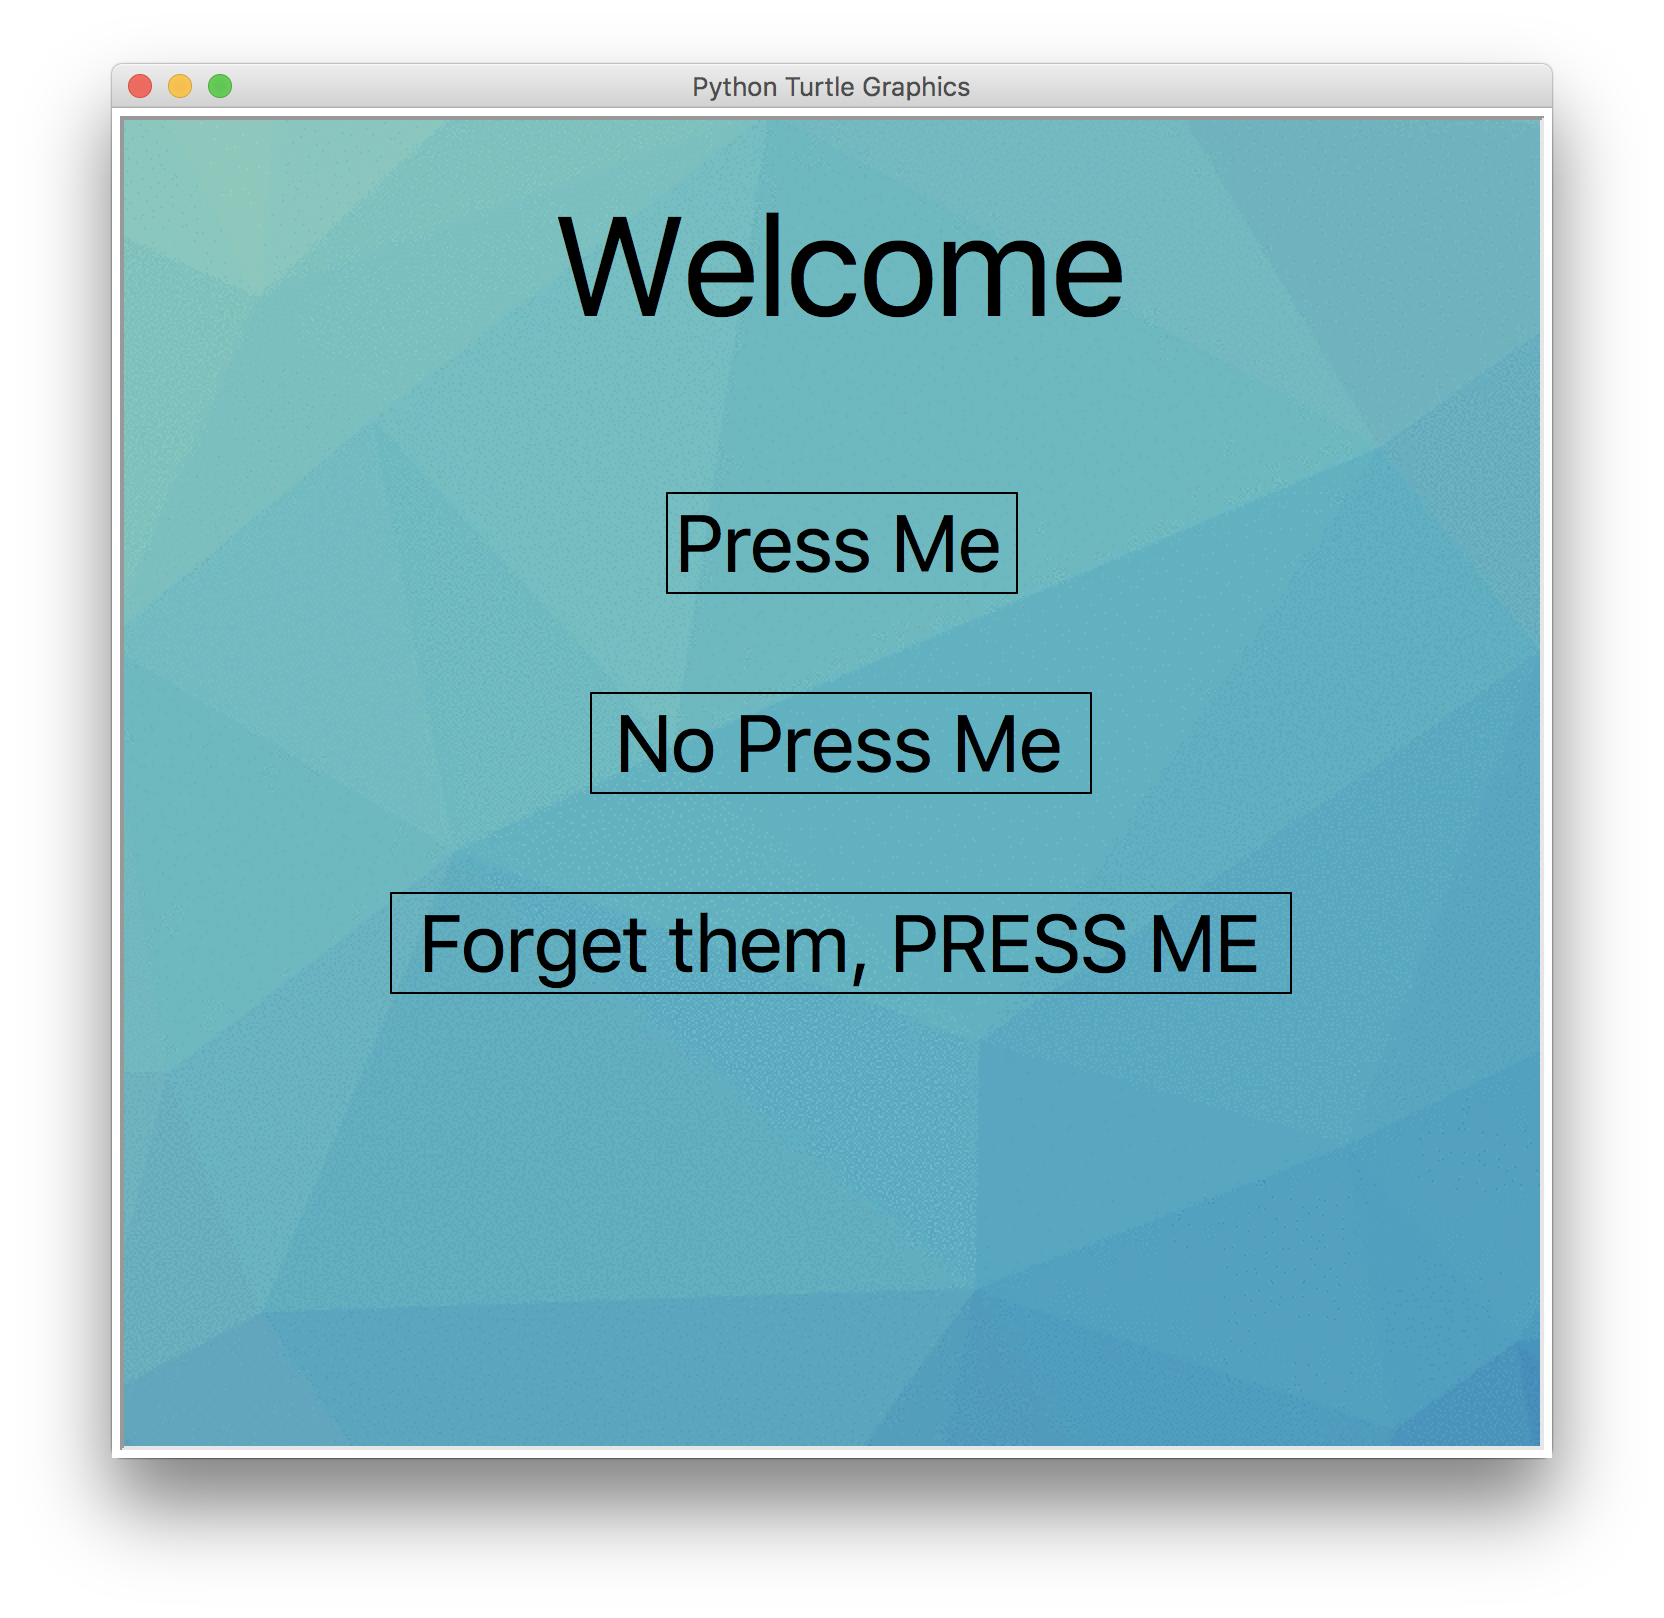
\includegraphics[width=4cm]{Menu_4}
}\hspace*{-1.5cm}

Now the above works, but putting basic drawing of a rectangle inside our draw button is not a great idea.  We will be drawing lots of rectangles so lets move that code out into a new helper function.

\TODO{Before your \code{drawButton} function in \code{Define helper functions} section, insert the following function}

\codeonly{title={\code{Menu.py}}}{31}{46}{code}{Menu_5.py}  

This function will draw a rectangle of width \code{w}, and height \code{h}, with bottom left corner at position (\code{x},\code{y}). You can also specify the border colour and the fill colour.

\vspace{12pt}

You should think about extending this function by, for example,
\begin{itemize}
\item Adding parameter \code{pensize=2} which would set the thickness of the border.
\item Adding parameter \code{shadow=False} which when set to \code{True} would draw a shadow. 

Drawing a shadow, is actual easy --- we just draw a few rectangles a little to the right an a little below the position of the main rectangle BEFORE we draw the main rectangle. If you are exceedingly lazy (this is a good thing in a programmer!) you can draw the shadow rectangles by just calling the \code{drawRectangle} function from inside the  \code{drawRectangle}
\end{itemize}
\newpage

Now your \code{drawButton can be simplified to}

\codeonly{title={\code{Menu.py}}}{49}{59}{code}{Menu_5.py}
\mbox{}\hfill\raisebox{0.85cm}[0pt][0pt]{%
	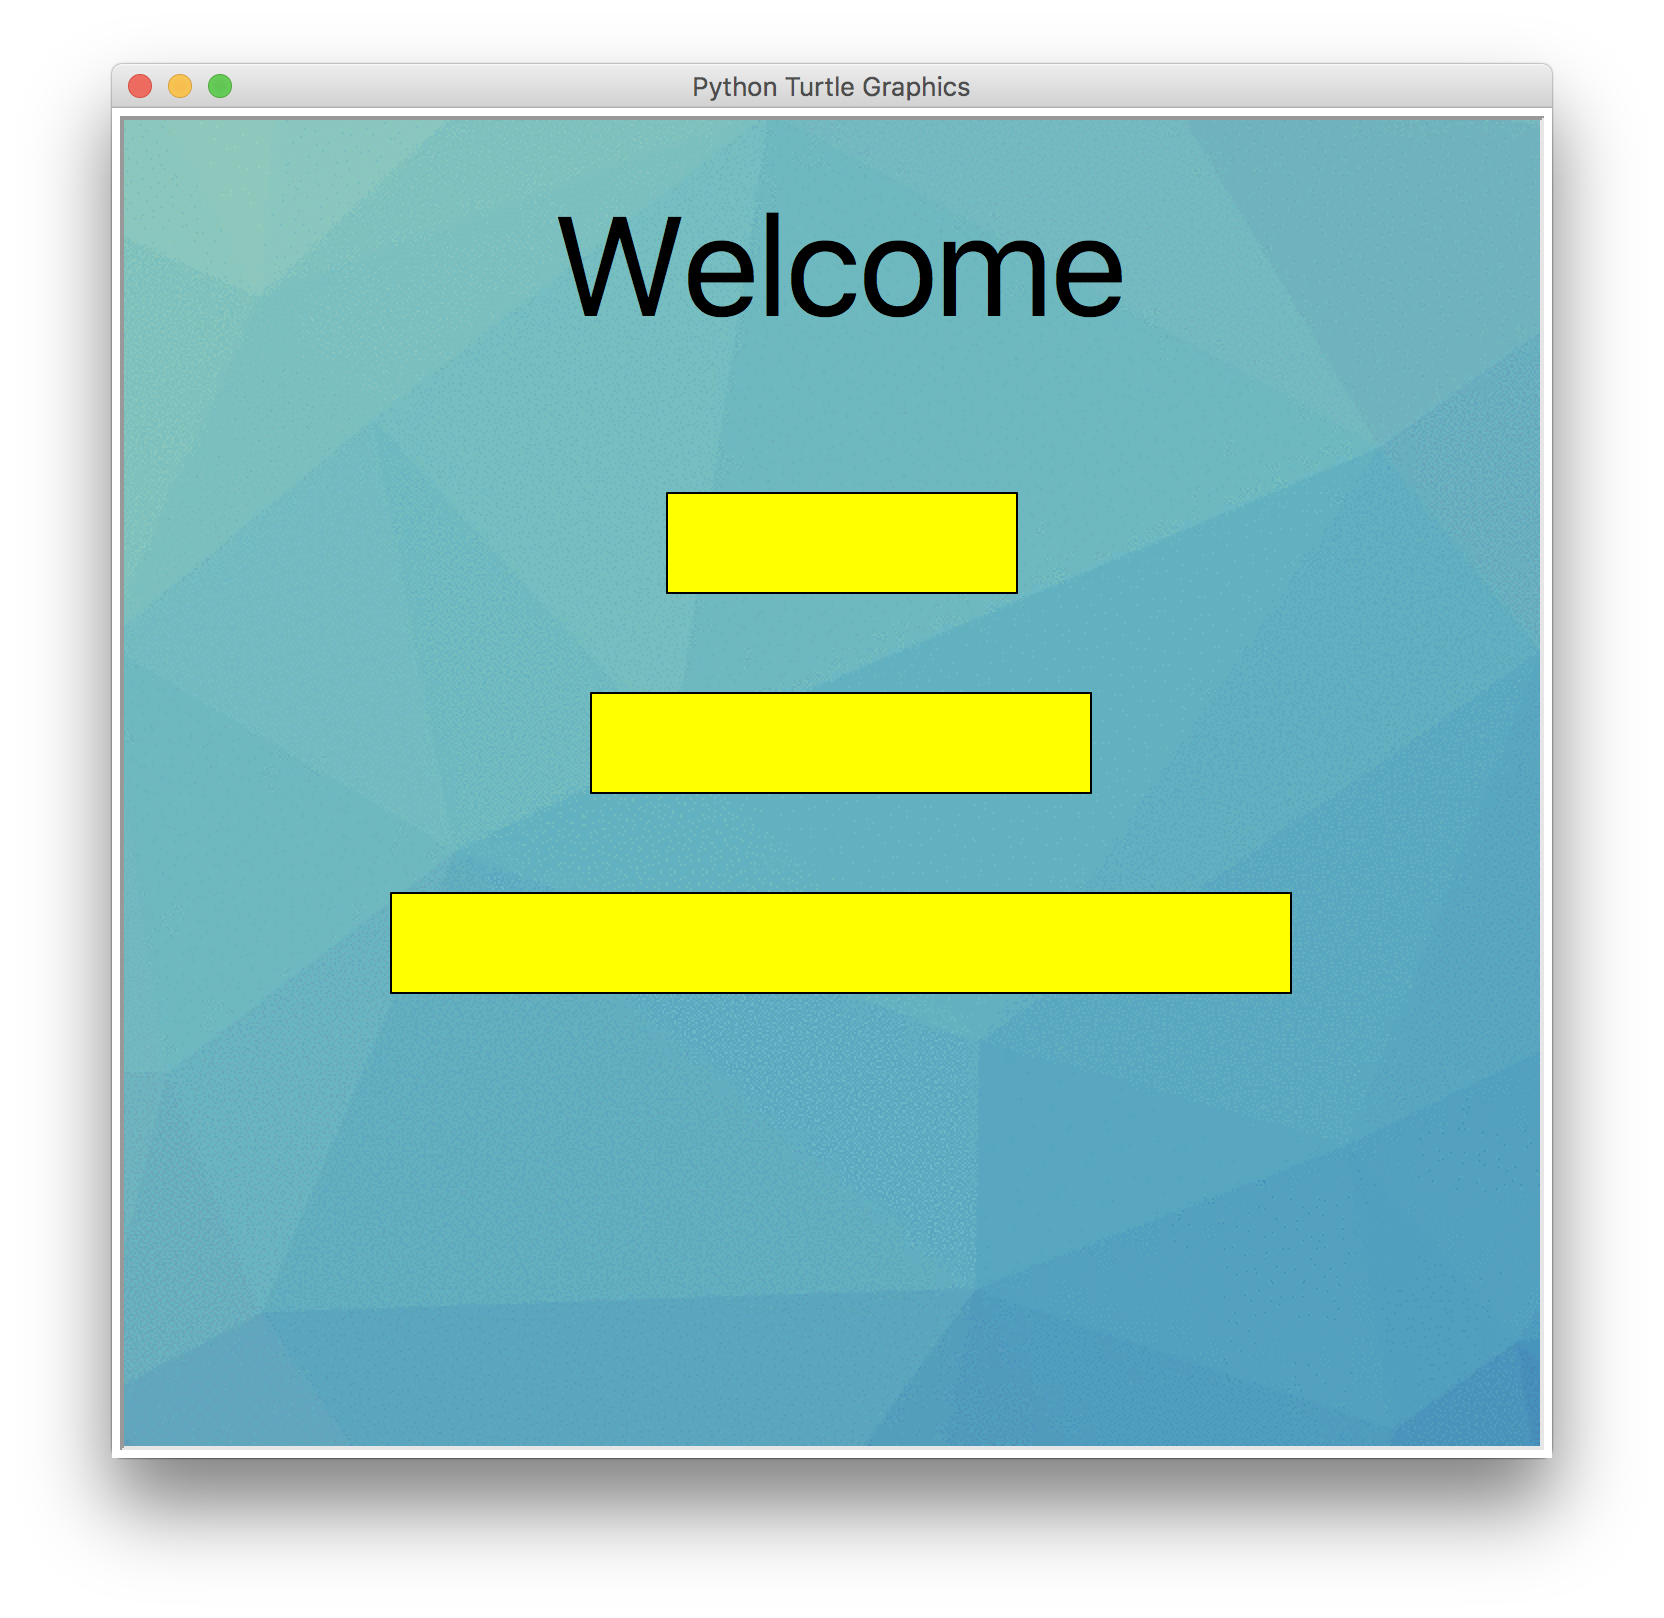
\includegraphics[width=4cm]{Menu_5}
}\hspace*{-1.5cm}

\TODO{If you look, really really carefully at the output you will see that {\em we} have done something silly.  To fix this, we need to draw the button label after drawing the border. Fix This.}

\codeonly{title={\code{Menu.py}}}{54}{64}{code}{Menu_6.py}
\mbox{}\hfill\raisebox{0.85cm}[0pt][0pt]{%
	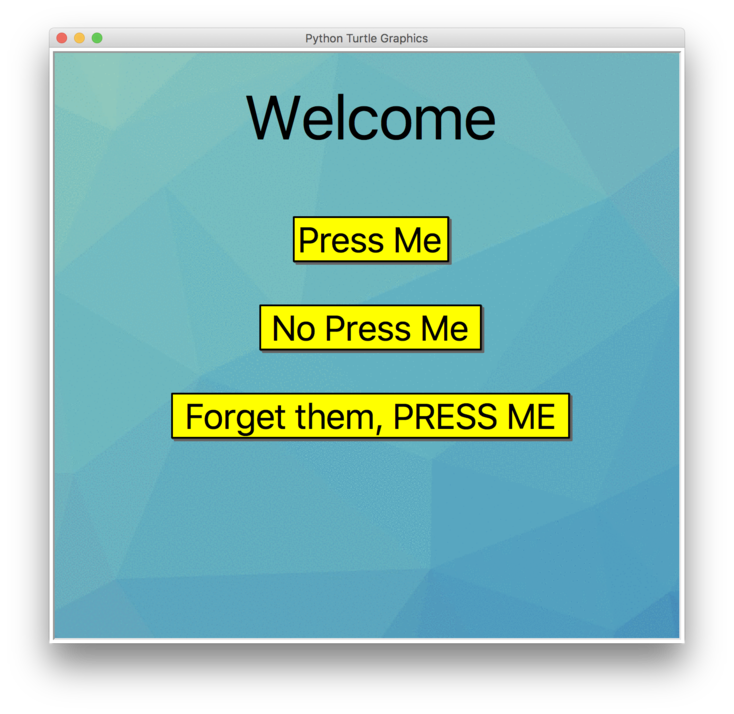
\includegraphics[width=4cm]{Menu_6}
}\hspace*{-1.5cm}


\subsubsection{Making the buttons work}

OK, now we have things that looks like buttons, but they do not act like them --- click on a button and see what happens --- nothing. 

To get the buttons to work we need to do two things:

\begin{itemize}
\item Listen for and respond to click events.

This is easy --- we will create our own \code{onclick} function to run whenever the user clicks on the screen.

\item When a click occurs, decide whether it happened within a button region and which button.

This is a little harder so we will talk about this in some detail.
\end{itemize}

\newpage

\TODO{Insert the following function at the bottom of the ``\code{Define helper functions}'' section of your code.}

\codeonly{title={\code{Menu.py}}}{67}{69}{code}{Menu_7.py}

and just before the \code{turtle.mainloop()} insert the lines

\codeonly{title={\code{Menu.py}}}{84}{85}{code}{Menu_7.py}

Now run your code and make sure you see a message appearing in {\em Thonny} every time you click the left mouse button. You should see that you also get the position of the mouse in the screen when the click occurred. Next we need to use this position information to determine which button was ``pressed''.

\TODO{Insert the code at the bottom of the ``\code{Create screen}'' section of your code.}

\codeonly{title={\code{Menu.py}}}{21}{23}{code}{Menu_8.py}

\begin{itemize}
\item
Lines 21 and 22, allow us to create an object (like the \code{Turtle} object or the \code{Screen} object) which stores information for a Button. Our \code{Button} object stores position (\code{x},\code{y}), size  \code{w} by \code{h}, and \code{label}.
\item
Line 23 defines an empty list, called \code{buttons}, that will store the information for all generated buttons.
\end{itemize}

So where do we get the information that we want to store in the \code{buttons} list?  

We have this information at end of \code{drawButton} function so that is where we will build our \code{Button} object.

\TODO{Modify the \code{drawButton} function so that it returns a \code{Button} object, as shown below.}
 
\codeonly{title={\code{Menu.py}}}{58}{69}{code}{Menu_8.py}

Now \code{bob} has a list of all of the generated buttons which we can search whenever the user clicks on the screen. First we need to make sure we are happy with our geometry. The mouse click is recorded at the point (\code{mx},\code{my}).  The conditions that must be true if this point is inside a button rectangle are shown in the following figure.

\begin{figure}[H]
\centering\larger[2]\vspace{-18pt}
\begin{tikzpicture}
	\draw[dashed,fill=yellow!20] (-5,0) rectangle (5,1.5);
	\fill[red] (0,0) circle (.1) node[below,black] {(\code{x},\code{y})};
	
	%\node[font={\larger[4]}]  at (0,0.75) {Press Me!};
	\draw[|-|] (5.5,0) -- node[fill=white] {\code{h}} ++(0,1.5); 
	\draw[|-|] (-5,1.8) -- node[fill=white] {\code{w}} ++(10,0); 
	\fill[blue] (-5,0) circle (.1) node[below,left,yshift=-9pt] 
	{(\code{x}-\code{w/2},\code{y})};
	\fill[blue] (5,1.5) circle (.1) node[above,right,yshift=12pt] {(\code{x+w/2},\code{y+h})};
	
	\fill[green!80!black] (3,1) circle (.1) node[below left,black] {(\code{mx},\code{my})};
	
	\draw[decorate,decoration={brace,amplitude=10pt}] (5,-1) -- 
	node[below, yshift=-15pt,fill=white,draw,drop shadow] 
	{\code{x}-\code{w/2 < mx <  x+w/2}}
	++(-10,0);

	\draw[decorate,decoration={brace,amplitude=10pt}] (-5.5,0) -- 
	node[left, xshift=-15pt, fill=white,draw,drop shadow] 
	{\code{y < my <  y+h}}
	++(0,1.5);
	
\end{tikzpicture}
\caption[Given button and point, determine if point is inside button]{Given a button and a point (\code{mx},\code{my}), determine if point is inside button.\label{fig:button}}
\end{figure}

\TODO{Modify your \code{onclick} function so that it check every button stored in \code{bob.buttons} using the conditions on (\code{mx},\code{my}) shown in the above figure.\\

Run this code and verify that whenever you click on a button that button's label is printed.
}

\codeonly{title={\code{Menu.py}}}{72}{78}{code}{Menu_8.py}


So finally we want to run different code depending on which button has been pressed. To do this we check the label of the button.

\TODO{Update the \code{onclick} function as shown below.}

\codeonly{title={\code{Menu.py}}}{72}{87}{code}{Menu_9.py}

\subsection{It's Lego time --- Putting your Programs Together}

OK, we now have nearly everything to build our menu. To get the menu layout that I showed at the start of this worksheet I used the following code.  You don't have to follow this.

\codeonly{title={\code{Menu.py}}}{99}{118}{code}{Menu_10.py}
\mbox{}\hfill\raisebox{7cm}[0pt][0pt]{%
	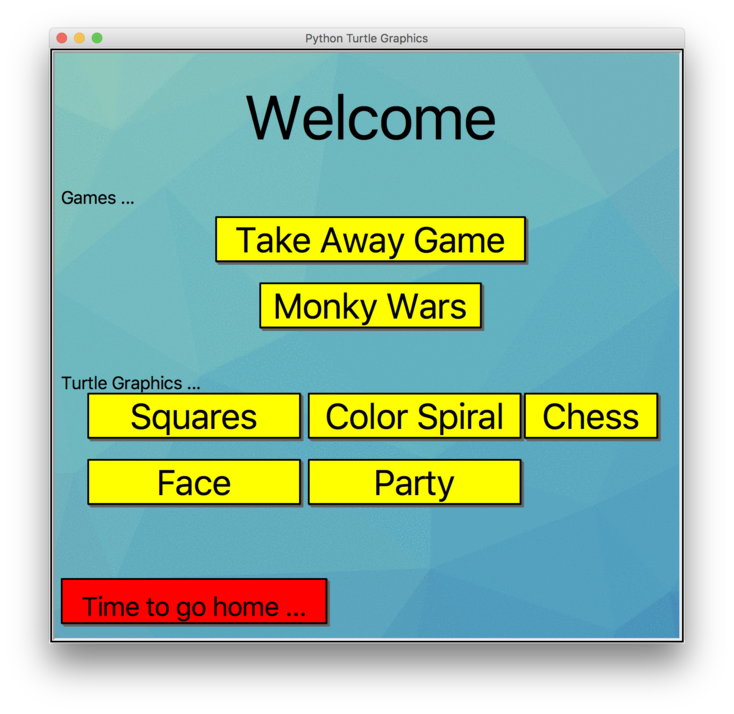
\includegraphics[width=6cm]{Menu_Complete}
}\hspace*{-1.5cm}

Then in my \code{onclick} functions I have added {\bf some} of the code needed to respond to the above button clicks.
 
\codeonly{title={\code{Menu.py}}}{72}{89}{code}{Menu_10.py}

Notice in line 80 and in line 83 I run other python files.  You will need to change this to match the name that you used for your files.
\end{document}




